\documentclass[11pt,a4paper,article,oneside]{memoir}
\usepackage{amsmath,amssymb,color,tikz,pgfplots}
\usepgfplotslibrary{groupplots}
\counterwithout{section}{chapter}
\DeclareMathOperator{\Hc}{h.c.}  \DeclareMathOperator{\Tr}{Tr}
\newcommand{\Gap}{\,\,\,\,\,\,\,\,\,} \newcommand{\Ua}{\uparrow}
\newcommand{\Da}{\downarrow} \newcommand{\hh}[1]{\hat{#1}}
\newcommand{\bra}[1]{\left\langle #1\right|}
\newcommand{\ket}[1]{\left| #1\right\rangle}
\newcommand{\expt}[2]{\left\langle #1| #2\right\rangle}
\newcommand{\outr}[2]{\left| #1\right\rangle\left\langle #2\right|}
\newcommand{\proj}[1]{\outr{#1}{#1}}
%
\begin{document}
\section{Master equation for a dissipative spin-chain}
%% \begin{figure}
%%   \includegraphics[width=\textwidth]{marcoscav}
%%   \caption{An array of coupled optical cavities, with losses from
%%     each site. The cavities are assumed to be highly non-linear, which means
%%     the effective occupation of photons at each site is limited to the
%%     $n=0,1$ subspace. The cavities are be driven to keep the photon number
%%     non-zero. Losses are characterised by the rate $\Gamma$.
%%     The effective Hamiltonian is that of
%%     a nearest-neighbour coupled spin-chain. (Figure taken from \cite{Marcos2012}: D. Marcos, A. Tomadin, S. Diehl, and P. Rabl. Photon condensation in circuit quantum electrodynamics by engineered dissipation. \textit{New J. Phys.}, \textbf{14}, 2012.)}
%%     \label{fig:coupledcavities}
%% \end{figure}
The project will mainly focus on a particular many-body quantum
system, that of an array of optical cavities, with nearest-neighbour
coupling. Additionally, these cavities will have strong
non-linearities, restricting the local basis to a two-level
approximation (see Figure \ref{fig:coupledcavities}). Great interest
lies in the non-equilibrium dynamics of driven-dissipative optical
cavities. The reason for this is the rich non-equilibrium phase
diagrams, with novel non-equilibrium phase transitions
\cite{Diehl2008,Diehl2010,Marcos2012}.
\par It can be shown (see [...]) that coupled non-linear optical
cavities can replicate spin-chain physics. This comes about when the
cavities have stong Kerr nonlinearities. Consider an array of $N$
coupled non-linear optical cavities, decribed by the Hamiltonian
\begin{equation}
  H_{cc}=\sum_i \omega_0 a^\dagger_ia_i - J
  \sum_i(a^\dagger_ia_{i+1}+a_ia^\dagger_{i+1}) +
  \frac{U}{2}\sum_{i}a^\dagger_ia^\dagger_ia_ia_i.
\end{equation}
Here, $a^\dagger_i$ and $a_i$ create or destroy a photon in the
$i^\text{th}$ cavity. The sum runs over all $N$ cavity labels,
$i$. The bare cavity frequency is $\omega_c$ and the non-linearity is
decribed by an interaction strength $U$. Finally, neighbouring
cavities may interact with one another, with a hopping strength
$J$. The spin physics is emulated in the regime where the energy
associated with the non-linearity is far above all other energy
scales, namely $\omega_c,t\ll U$. This restricts the population of
photons on each site to either $1$ or $0$.  Correspondingly, the
physics is effectively decribed by a chain of spins, with an effective
Hamiltonian of the form
\begin{equation}
  H_{eff}=\sum_i\omega_0 \sigma^z_i -J \sum_i
  (\sigma^+_i\sigma^-_{i+1}+\sigma^+_i\sigma^-_{i+1}).
\end{equation}
In this Hamiltonian, we are now describing the occupation of a site in
a spin language, with an up-spin corresponding to the presence of a
photonic excitation and a down-spin corresponding to no
excitation. $\sigma^z_i$ is the Pauli operator acting in the $z$
quadrature, and $\sigma^\pm_i$ is a spin raising(lowering) operator,
written in terms of the $x$- and $y$-spin Pauli operators as
$\sigma^\pm_i=\sigma^x_i\pm i\sigma^y_i$. Because this system has
site-to-site coupling, the resulting eigenstates are inherently
non-local.  \par The cavities also dissipate into their environment,
and are driven such that the photon population is above zero. The
exact nature of this dissipation depends on the physical processes,
and there are many frameworks to treat dissipation. This report
focuses on the application of a quantum master equation to describe
the dissipation. A master equation is the governing equation of motion
for the coupled-cavity quantum system, in the presence of
environmental dissipation and driving. Typically, a phenominologically
motivated master equation is written down, without considering a
detailed model for the system-bath interaction. For example, it may be
the case that each of the optical cavities is imperfect, and that they
each leak light into their environment. A rate of loss, $\Gamma$ can
be introduced, which characterises the dissipation from each site,
independently of one another. This is justified in certain optical
regimes \cite{hartmann}, and has been shown to display photon
crystallisation even in the presence of the losses and a coherent
drive.  \par The non-equilibrium physics that emerges maintains
long-range order in its steady states, despite the incoherent loss
from each cavity. The question then is: \textit{what results by
  considering all normal-modes in the dissipation, not simply
  site-independent dissipation?} This project investigates the result
of correctly treating dissipation by expanding in a basis of the spins
Hamiltonian, in the regime of a zero-temperature environment. We
consider a special case of a system-environment coupling, in a
rotating wave approximation, which preserves total excitation number
in the composite system-environment quantum system.  \par \par In this
section, we introduce a general model for a chain of spins, each
coupled to their own environment. By considering a special form of the
system-environment interaction, we derive a master equation which
takes account of the full dissipative dynamics. This is acheived by
not simply introducing independent decay terms, but by starting with a
composite system-environment quantum system and calculating the master
equation for the reduced system density matrix.
%
\subsection{Model}
The most general class of models one may write down to describe a
chain of interacting spins is the fully anisotropic Heisenberg (or
XYZ-) model. This is represented by the Hamiltonian:
\begin{equation}
  H_S = -J\sum_{i=1}^N
  \left(\Delta_x\sigma^x_i\sigma^x_{i+1}+\Delta_y\sigma^y_i\sigma^y_{i+1}+
  \Delta_z\sigma^z_i\sigma^z_{i+1}+\frac{g}{J}\sigma^z_i\right),
\end{equation}
where $\sigma^x_i$, $\sigma^y_i$ and $\sigma^z_i$ are Pauli operators
describing the spin degree of freedom at site $i$. The dimensionless
parameters $\Delta_x$, $\Delta_y$ and $\Delta_z$ describe the
anisotropic, nearest-neighbour spin-spin interaction strength.
Finally, an external field which tends to align the spins in the
$z$-spin direction has be added with an associated energy scale of
$g$. Finally, $t$ is the hopping parameter, describing the strength of
the internal system interactions. 
\par Periodic boundary
conditions (where we set $\sigma^\gamma_1=\sigma^\gamma_{N+1}$, for all
$\gamma=x,y,z$) may or may not be adopted. In this report the choice
will be stated before any relevant calculation.
\par The
\textit{closed} system dynamics of the system $S$ are captured by the
unitary evolution generated by the Hamiltonian. As such, states of
system $S$, $\ket{\psi}_S$ obey the Schr\"odinger equation
$i\partial_t\ket{\psi}_S=H_S\ket{\psi}_S$ (where $\hbar=1$). However,
this form of the dynamics is not the main concern of this report. The
further influence on the system due to an array of environments, $E$
is considered. Suppose that each lattice site in the chain of spins is
coupled to a local thermal reservoir, denoted $B_i$ (see figure
\ref{fig:dissspinchain}). Each reservoir is modelled as an harmonic
oscillator, so that the free evolution of the environmental degrees of
freedom is captured by the Hamiltonian (the terms bath, reservoir and
environment are used interchangeably):
\begin{equation}
  H_B = \sum_{i=1}^N\sum_k\omega_kb^\dagger_{i,k}b_{i,k}.
\end{equation}
\begin{figure}[t]
  \begin{center}
    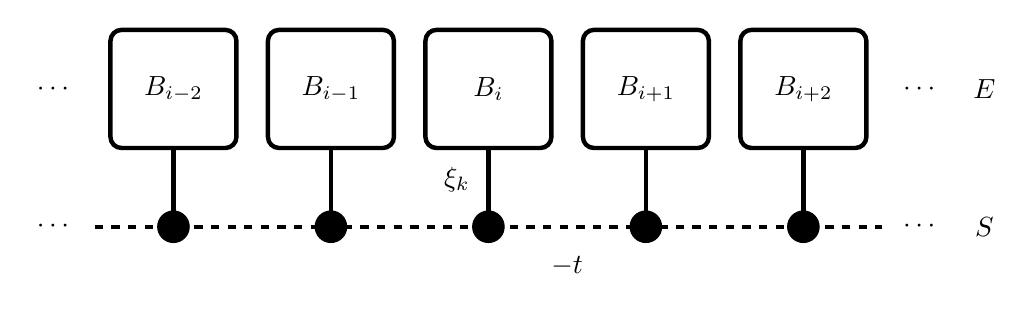
\begin{tikzpicture}
      \draw [dashed, ultra thick] (-5,0) -- (5,0); \draw [fill] (-4,0)
      circle [radius=0.2]; \draw [fill] (-2,0) circle [radius=0.2];
      \draw [fill] (0,0) circle [radius=0.2]; \draw [fill] (2,0)
      circle [radius=0.2]; \draw [fill] (4,0) circle [radius=0.2];
      \draw [ultra thick] (-4,0) -- (-4,1); \draw [ultra thick] (-2,0)
      -- (-2,1); \draw [ultra thick] (0,0) -- (0,1); \draw [ultra
        thick] (2,0) -- (2,1); \draw [ultra thick] (4,0) -- (4,1);
      \draw [ultra thick, rounded corners] (-4.8,1) rectangle
      (-3.2,2.5); \draw [ultra thick, rounded corners] (-2.8,1)
      rectangle (-1.2,2.5); \draw [ultra thick, rounded corners]
      (-0.8,1) rectangle (0.8,2.5); \draw [ultra thick, rounded
        corners] (1.2,1) rectangle (2.8,2.5); \draw [ultra thick,
        rounded corners] (3.2,1) rectangle (4.8,2.5); \node at (-4,
      1.75) {$B_{i-2}$}; \node at (-2, 1.75) {$B_{i-1}$}; \node at (0,
      1.75) {$B_{i}$}; \node at (2, 1.75) {$B_{i+1}$}; \node at (4,
      1.75) {$B_{i+2}$}; \node at (1,-0.5) {$-t$}; \node at (-0.4,0.6)
      {$\xi_k$}; \node at (5.5,0) {$\cdots$}; \node at (5.5,1.75)
      {$\cdots$}; \node at (-5.5,0) {$\cdots$}; \node at (-5.5,1.75)
      {$\cdots$}; \node at (6.3,0) {$S$}; \node at (6.3,1.75)
      {$E$};
    \end{tikzpicture}
    \caption{A schematic of the dissipative spin chain considered in
      this project. A chain of two-level systems (spin-$\frac{1}{2}$
      particles) are coupled to their nearest-neighbours and to a
      local environment, with coupling strength parameters
      $\xi_k$. The environments are modelled as bosonic harmonic
      oscillators.}
    \label{fig:dissspinchain}
  \end{center}
\end{figure}The $b_{i,k}$ are the bosonic annihilation operators for the
$i^\text{th}$ site, $k^\text{th}$ mode and $\omega_k$ is the energy of
a particle in the $k^\text{th}$ mode. The baths are assumed to be
identical (in that they each have the same $\omega_{k}$) but are
otherwise isolated from one another. This means that the canonical
commutation relations for the bath operators are
$[b_{i,k},b_{j,q}]=[b^\dagger_{i,k},b^\dagger_{j,q}]=0$ and
$[b_{i,k},b^\dagger_{j,q}]=\delta_{i,j}\delta_{k,q}$. Within this
framework, with a system of interest coupled to a large environment,
the system of spins becomes an \textit{open quantum system} (see
Figure \ref{fig:open}). In the theory of open quantum systems
\cite{Breuer2002} one wants to determine the laws of motion for the
reduced system dynamics. This involves tracing over the environments
to determine $\dot{\rho}_S(t)$, the rate of change of the partially
traced density matrix $\rho_S=\Tr_B\{\rho_S\}$.
\subsection{System-bath interaction}
We are now in position to put the all the elements of a dissipative
array of optical cavities. All that is left is to describe the
specific interaction between the system and environment. When the
array dissipates into an environment, there needs to be a drive to
keep the population non-zero. We follow \cite{Biella2015, Genway2014,
  Joshi2013} and consider a coherent drive, which creates pairs of
photons in neighbouring cavities. The driven Hamiltonian has a time
dependence, and in the spin language is given by
\begin{align}
  H&=\sum_i\omega_0 \sigma^z_i -J \sum_i
  (\sigma^+_i\sigma^-_{i+1}+\sigma^+_i\sigma^-_{i+1})
  \notag\\ &-\Omega\sum_i\left(\sigma^+_i\sigma^+_{i+1}
  e^{-2i\omega_Pt}+\sigma^-_i\sigma^-_{i+1}e^{2i\omega_Pt}\right).
\end{align}
The additional non-number-conserving terms
$\sigma^+_i\sigma^+_{i+1}e^{-2i\omega_Pt}$ and
$\sigma^-_i\sigma^-_{i+1}e^{2i\omega_Pt}$ represent the external
coherent drive, which has strength $\Omega$. Finally, we model
dissipation by introducing an interaction with a set of
environments. This interaction is assumed to be of the form
\begin{equation}
  H_I=\sum_i \sum_k \xi_k \sigma^x_i \otimes (b_{i,k}+b^\dagger_{i,k}).
\end{equation}
\par It is convenient to move into a rotating frame with repect to the
driving frequency. When we do this the system operator in the
coupling, $\sigma^x_i$ gains a time-dependence and the interaction can
we written
\begin{equation}
  H_I=\sum_i \sum_k
  \xi_k\left(\sigma^+_ib_{i,k}+\sigma^-_ib^\dagger_{i,k}+\sigma^+_ib^\dagger_{i,k}e^{-2i\omega_Pt}+\sigma^-_ib_{i,k}e^{2i\omega_Pt}\right).
\end{equation}
The common assumption, and the assumption we make in this work is that
the pump frequency is well above the bare cavity frequency $\omega_0$,
and the hopping strength $J$. This means that the fast oscillating
terms $\sigma^+_ib^\dagger_{i,k}e^{-2i\omega_Pt}$ and
$\sigma^-_ib_{i,k}e^{2i\omega_Pt}$ can be neglected due to
averaging. The final interaction in the rotating frame has the simple
form
\begin{equation}
  H_I = \sum_i \sum_k \xi_k (\sigma+_ib_{i,k}+\sigma^-_ib^\dagger_{i,k}).
\end{equation}
It is straight-forward to demonstrate that in the rotating frame the
Hamiltonian above becomes
\begin{align}
  H&=\sum_i(\omega_0-\omega_P) \sigma^z_i -J \sum_i
  (\sigma^+_i\sigma^-_{i+1}+\sigma^+_i\sigma^-_{i+1}),
\end{align}
with the environments' Hamitlonian being similarly transformed:
\begin{equation}
  H_B = \sum_{i=1}^N\sum_k(\omega_k-\omega_P)b^\dagger_{i,k}b_{i,k}.
\end{equation}
The total system-environment Hamiltonian takes the final form
\begin{align}
  H &= H_S + H_B + H_I \notag \\ &= \sum_i(\omega_0-\omega_P)
  \sigma^z_i-J\sum_{i=1}^N
  \left(\sigma^+_i\sigma^-_{i+1}+\sigma^+_i\sigma^-_{i+1}\right)
  \notag
  \\ &\Gap+\sum_{i=1}^N\sum_k(\omega_k-\omega_P)b^\dagger_{i,k}b_{i,k}
  + \sum_i \sum_k \xi_k (\sigma+_ib_{i,k}+\sigma-_ib^\dagger_{i,k}).
\end{align}
This model now contains all the elements to develop an open quantum
theory. All that remains is that we calculate the dynamical equation
of motion for the system of cavities.
\begin{figure}
  \begin{center}
    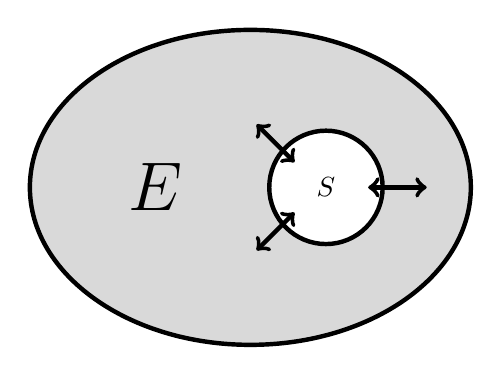
\begin{tikzpicture}[scale=0.8]
      \draw [fill=gray!30,ultra thick] (-2,0) ellipse (3.5 and 2.5);
      \node at (-3.5,0) {{\Huge $E$}}; 
      \draw [fill=white,ultra thick] (-0.8,0) circle [radius=0.9]; 
      \node at (-0.8,0) {$S$};
      \draw [<->, ultra thick] (-1.3, 0.4) -- (-1.9,1);
      \draw [<->, ultra thick] (-1.3, -0.4) -- (-1.9,-1);
      \draw [<->, ultra thick] (-0.13, 0) -- (0.8,0);
    \end{tikzpicture}
  \end{center}
  \caption{A representation of an open quantum system. A system of
    interest $S$ is influenced by its surrounding environment, $E$. We
    assume that this influence can be represented by an interaction
    term in the Hamiltonian, $H_I$.}
  \label{fig:open}
\end{figure}
\subsection{Equation of motion for $S$}
\par In the Schr\"odinger picture, the equation of motion for the
density matrix of the compsite system $S+E$ is given by the equation:
\begin{equation}
  \dot{\rho}=-i[H,\rho].
\end{equation}
In an open quantum system, one traces over the environment, and is
left with an equation of motion for the reduced system density matrix
$\rho_S$ of the form
\begin{equation}
  \dot{\rho}_S=-i[H_S,\rho_S]+\mathcal{D}\rho_S.
\end{equation}
The term $\mathcal{D}\rho_S$ is known as a dissipator of the dynamics
and decribes a generalised relaxation process. We are intersted in
deriving a form for $\mathcal{D}\rho_S$ from \textit{first
  principles}. Often, what is done to arrive at an equation like the
one above is that a form for the dissipator is chosen based of
phenomenological reasoning. In particular, often a dissipator in
Lindblad form
\begin{equation}
  \mathcal{D}[a]\rho_S=a\rho_Sa^\dagger-\frac{1}{2}\{a^\dagger a,
  \rho_S\}
\end{equation}
is chosen. The operator $a$ is a system operator, and is refered to as
a \textit{jump} operator. A dissipator in Lindblad form generates a
form of dynamics which is trace preserving, and crucially, completely
positive.  \par To derive the form of $\mathcal{D}$ from scratch we
take the standard approach of deriving a Born-Markov master equation
in a weak system-environment coupling regime. Let us first move into
an interaction picture, so that kets have a time dependence generated
by the `free' Hamiltonian $H_S+H_E$, with operator's time dependence
being generated by the interaction Hamiltonian $H_I(t)$ (see
\cite{Breuer2002} for a complete description of the interaction
picture). In the interaction picture, the equation of motion for the
density matrix of $S+E$ is the von Neumann equation:
\begin{equation}
  \dot{\rho}(t)=-i[H_I(t),\rho(t)].
  \label{eqn:vonNeumann}
\end{equation}
The trace over the environment then may be taken, to obtain an
equation of motion for just the system of interest, $S$:
\begin{equation}
  \dot{\rho}_S(t)=-i\Tr_B[H_I(t),\rho(t)].
  \label{eqn:vonNeumann2}
\end{equation}
It is in general exceedingly difficult to work with the von Neumann
equation directly, as the step of tracing the environment has a
dependence on the full composite system density matrix, $\rho(t)$. It
is thus necessary to look for approximations to the RHS of Equation
(\ref{eqn:vonNeumann2}).  \par One common set of approximations is the
combination of the Born approximation and the Markov approximation
which, when combined, convert the RHS of Equation
(\ref{eqn:vonNeumann2}) into a Born-Markov master equation. Firstly,
we formally integrate Equation (\ref{eqn:vonNeumann}). This then gives
us a closed form for the density matrix
$\rho(t)=-i\int^tds[H_I(s),\rho(s)]$, which then may be substitured
back into the von Neumann equation, resulting in
\begin{equation}
  \dot{\rho}(t)=-\int^tds[H_I(t),[H_I(s),\rho(s)]].
  \label{eqn:master1}
\end{equation}
This process can of course be repeated \textit{ad infinitum}, by
formally integrating and substituting, resulting in higher and higher
orders of perturbation theory. As was mentioned above, we are going to
work in the weak coupling regime, and so stop this process after one
formal integration and subtitution.  \par The Born approximation says
that the system and environment are sufficiently weakly coupled such
that the total density matrix may be written as a product
$\rho(t)=\rho_S(t)\otimes\tilde{\rho}_B$. The environment is assumed
to be sufficiently large such that the weak interaction with system
does not perturb its state. We denote the time-constant environmental
density matrix $\tilde{\rho}_B$. This can take many forms, for example
a thermal state
\begin{equation}
  \tilde{\rho}_B=\prod_{i,k}\frac{e^{-\beta\omega_{k}
      b^\dagger_{i,k}b_{i,k}}}{\mathcal{Z}},
      \label{eqn:thermal}
\end{equation}
where $\beta=1/k_BT$ is the inverse temperature and
$\mathcal{Z}=\sum_{i,k}e^{-\beta\omega_k}$ is the partition
function. Under asssumption the master equation (\ref{eqn:master1})
takes the form, after tracing over the baths
\begin{equation}
  \dot{\rho}_S(t)=-\int^tds\Tr_B[H_I(t),[H_I(s),\rho_S(s)\otimes\tilde{\rho}_B]].
\end{equation}
\par Now the Markov approximation is made, assuming there is no
`history dependence' of the system on its previous states (time
locality). The following modifications to the above master equation
are made. First, we remove the history dependence by replacing
$\rho_S(s)\rightarrow\rho_S(t)$. Next the limit on the integral is
taken to infinity, while the replacement $H_I(s)\rightarrow H_I(t-s)$,
so that the integral has no dependence on the initial time.  Without
loss of generality, we let $t=0$ be the time at which the system is
set up. So the final Born-Markov master equation
\begin{equation}
  \dot{\rho}_S(t)=-\int^\infty_0ds\Tr_B[H_I(t),[H_I(t-s),\rho_S(t)\otimes\tilde{\rho}_B]].
  \label{eqn:bornmark}
\end{equation}
This equation thus determines the dynamics of the system $S$, whilst
taking account of the irreversible losses to an environment. Keeping
track of all the environmental degrees of freedom is no longer
required, an assumption about the state of the environment is all the
remains. This would then allow one to evaluate the trace $\Tr_B$ and
time integral, as we will now demonstrate.
\subsection{Dissipation from first principles}
\par One particularly useful and general approach to the evaluation of
the RHS of the Born-Markov master equation is to introduce a set of
eigenoperators of the system Hamiltonian $H_S$. (This method is
outlined in the text book \textit{The Theory of Open Quantum Systems}
by Breuer and Petruccione.) \par The aim in this project is to
calculate the full dissipation the interaction picture we have that
\begin{equation}
	H_I(t) = e^{i(H_S+H_E)t}H_I(0)e^{-i(H_S+H_E)t}.
\end{equation}
Given a general $H_I$, this is not easy to calculate explicitly the
time dependence without the help of the system eigenoperators, which
we now introduce.  \par Suppose we fully understand the system and
environment seperately, that is, we know how to calculate the system
and environment eigenspectrums (this may be always achieved in
principle by numerical diagonalisation) then we may express a
resolution of identity in the following manner (the system alone for
simplicity):
\begin{equation}
\mathcal{I}_S=\sum_{\substack{\forall \epsilon\,\text{s.t.}
    \\ H_S\ket{\epsilon}=\epsilon\ket{\epsilon}}}\outr{\epsilon}{\epsilon}.
\end{equation}
The equivalent expression for the baths is simply the sum of outer
products of Fock basis states (since we model the environment as a
system of oscillators). With the assumption that the interaction is
seperable: $H_I = \sum_i A_i \otimes B_i$, this then allows direct
calculation of the interaction Hamiltonian in the interaction picture:
\begin{align}
H_I(t) &= \sum_i \sum_{\forall\epsilon,\forall\upsilon}
e^{iH_St}\outr{\epsilon}{\epsilon}A_i\outr{\upsilon}{\upsilon}e^{-iH_St}\otimes
B_i(t) \notag \\ &= \sum_i
\sum_{\forall\epsilon,\forall\upsilon}e^{i(\epsilon-\upsilon)t}\bra{\epsilon}A_i\ket{\upsilon}
\outr{\epsilon}{\upsilon}\otimes B_i(t) \notag
\\ &\equiv\sum_i\sum_{\forall\epsilon,\forall\upsilon}e^{i(\epsilon-\upsilon)t}A^i_{\epsilon,\upsilon}\otimes
B_i(t),
\end{align}
where $A^i_{\epsilon,\upsilon} = \bra{\epsilon}A_i\ket{\upsilon}
\outr{\epsilon}{\upsilon}$.  Sometimes it is convenient to rewrite
this as a single sum over possible energy-\textit{differences}, as
opposed to an explicit double sum over energy eigenvalues. To this
end, we introduce the energy eigenoperators of $S$:
\begin{equation}
	A^i_\omega=\sum_{\forall\epsilon,\forall\upsilon}\delta_{\omega,\epsilon-\upsilon}A^i_{\epsilon,\upsilon}.
\end{equation}
With this notation we may then write a single sum to denote sum over
all frequency differences, $\omega$ which gives:
\begin{align}
H_I(t) &=\sum_i\sum_{\omega}e^{i\omega t}A^i_\omega\otimes B_i(t).
\label{eq:intham}
\end{align}
We have thus expressed the interaction picture Hamiltonian in terms of
operators we may readily calculate with. In this technique it is
generally assumed that the environments are vast and can be
represented by harmonic oscillators. All expectations and correlations
of operators acting on such a bath written in terms of the bath's
creation and annihilation operators may be easily calculated. So the
complexity of such expressions as (\ref{eq:intham}) is due the unknown
form of the operators $A^i_\omega$. However, calculation of these
operators is necessary if we want to assure that the full dynamics due
to the system-environment coupling is accounted for.
\subsection{Non-local dissipation to a zero-temperature environment}
In this section a master equation with all non-local contributions
included is derived. To evaluate the RHS of the Born-Markov master
equation (\ref{eqn:bornmark}), the time dependence of the interaction
Hamiltonian $H_I(t)$ in the interaction picture must be
determined. One method of choice is to choose a basis of
eigenoperators of the system Hamiltonian $H_S$, and this is the
approach utilised in this report. Recall the number-conserving
interaction Hamiltonian between each spin-site and its unique
environment
\begin{equation}
	H_I=\sum_{i=1}^N\sum_k
        \xi_k\left(\sigma^+_ib_{i,k}+\sigma^-_ib^\dagger_{i,k}\right).
\end{equation}
This is can be expressed in terms of the eigenoperators of $H_S$ as
explained in the preceding section. This then gives the interaction
Hamiltonian:
\begin{equation}
	H_I(t)=\sum_{i,k}\sum_{\omega}\xi_k A^i_\omega
        b^\dagger_{i,k}(t)e^{i\omega t}+\Hc,
    \label{eqn:HIeigen}
\end{equation}
where $A^{i}_\omega =
\sum_{\epsilon,\upsilon}\delta_{\omega,\epsilon-\upsilon}A^{i}_{\epsilon,\upsilon}$
and $A^{i}_{\epsilon,\upsilon} =
\bra{\epsilon}\sigma^-_i\ket{\upsilon} \outr{\epsilon}{\upsilon}$. The
corresponding quantum master equation is obtained upon evaluation of
the right hand side of (\ref{eqn:bornmark}). This involves a double
commutator, which, since the interaction Hamiltonian has two terms,
will in general yield $16$ terms in the master equation. We are going
to neglect three quarters of these terms and calculate the
expectations with the assumption of empty baths (zero
temperature). Expectations with respect to a thermal density matrix,
such as (\ref{eqn:thermal}), are (where
$\langle\cdot\rangle=\Tr\{\cdot\,\tilde{\rho}_B\}$):
\begin{align}
	\Big\langle b_{i,k}b_{j,q}\Big\rangle = \left\langle
        b^\dagger_{i,k}b^\dagger_{j,q}\right\rangle &= 0,\notag
        \\ \left\langle b^\dagger_{i,k}b_{j,q}\right\rangle
        &=\delta_{i,j}\delta_{k,q}n(\omega_{k}),\notag\\ \left\langle
        b_{i,k}b^\dagger_{j,q}\right\rangle
        &=\delta_{i,j}\delta_{k,q}\left(n(\omega_{k})+1\right).
\end{align}
The following replacement is made for \textit{empty thermal
  reservoirs}: $n(\omega_{k})\rightarrow 0$, for all modes $k$. The
simplification is clear: since the only non-zero two-point correlator
is $\langle b_{i,k}b^\dagger_{j,q}\rangle =\delta_{i,j}\delta_{k,q}$,
many terms on the RHS of (\ref{eqn:bornmark}) are zero. With this in
mind the calculation of the dissipator will now be undertaken.  \par
Before turning the focus to the integral, the first step is to
evaluate the traced commutator
$\Tr_B[H_I(t),[H_I(t-s),\rho_S(t)\otimes\tilde{\rho}_B]]$ by inserting
the eigenoperator representation of $H_I(t)$ as given in
(\ref{eqn:HIeigen}).
\begin{align}
	\Tr_B[H_I(t),[H_I(&t-s),\rho_S(t)\otimes\tilde{\rho}_B]],\notag \\ 
	=\sum_{i,j}\sum_{k,q}\sum_{\omega,\omega'}\Tr_B&[\xi_k A^i_\omega
        b^\dagger_{i,k}(t)e^{i\omega t}+\Hc\,,[\xi_q A^{j}_{\omega'}
        b^\dagger_{j,q}(t-s)e^{i\omega' (t-s)}+\Hc\,,\rho_S(t)\otimes\tilde{\rho}_B]], \notag \\
	=\sum_{i,j}\sum_{k,q}\sum_{\omega,\omega'}\Tr_B&([\xi_k A^i_\omega
        b^\dagger_{i,k}(t)e^{i\omega t},[\xi_q A^{j,\dagger}_{\omega'}
        b_{j,q}(t-s)e^{-i\omega' (t-s)},\rho_S(t)\otimes\tilde{\rho}_B]]\notag \\
	&+[\xi_k A^{i,\dagger}_\omega
        b_{i,k}(t)e^{-i\omega t},[\xi_q A^{j}_{\omega'}
        b^\dagger_{j,q}(t-s)e^{i\omega' (t-s)},\rho_S(t)\otimes\tilde{\rho}_B]]).
        \label{eqn:doubcomm1}
\end{align}
The second to third line step in (\ref{eqn:doubcomm1}) follows by
dropping terms which generate traces of the form
$\Tr\{b^\dagger_{i,k}(t)b^\dagger_{j,q}(t-s)\tilde{\rho}_B\}$ and
$\Tr\{b_{i,k}(t)b_{j,q}(t-s)\tilde{\rho}_B\}$, which are each exactly
zero for bosonic particles.  \par The master equation can now be
expressed as \footnote{Note that the hermitian conjugate can be
  written since $[A,[A^\dagger,h]]^\dagger=[A^\dagger,[A,h]]$ if
  $h=h^\dagger$.}
\begin{align}
\dot{\rho}_S(t)=-\int^\infty_0ds\sum_{i,j}\sum_{k,q}\sum_{\omega,\omega'}\Tr_B[\xi_k A^i_\omega
        b^\dagger_{i,k}(t)&e^{i\omega t},[\xi_q A^{j,\dagger}_{\omega'}
        b_{j,q}(t-s)e^{-i\omega' (t-s)},\rho_S(t)\otimes\tilde{\rho}_B]] \notag \\
+\Hc
\end{align} 
We now expand the double commutator as $[A,[B,C]]=ABC-ACB-CBA+BCA$ and separate the system operators from the bath operators:
\begin{align}
  \dot{\rho}_S(t)=-\int^\infty_0ds\sum_{i,j}\sum_{k,q}\sum_{\omega,\omega'}&e^{i(\omega-\omega')t}e^{i\omega's}\xi_k\xi_q
  \notag\\ \times\Big(& A^i_\omega
  A^{j,\dagger}_{\omega'}\rho(t)\Tr_B\{b^\dagger_{i,k}(t)b_{j,q}(t-s)\tilde{\rho}_B\}
  \notag \\ -
  &A^i_\omega\rho(t)A^{j,\dagger}_{\omega'}\Tr_B\{b^\dagger_{i,k}(t)\tilde{\rho}_Bb_{j,q}(t-s)\}\notag
  \\ -&
  A^{j,\dagger}_{\omega'}\rho(t)A^i_\omega\Tr_B\{b_{j,q}(t-s)\tilde{\rho}_Bb^\dagger_{i,k}(t)\}\notag
  \\ +&\rho(t)A^{j,\dagger}_{\omega'}A^i_\omega\Tr_B\{\tilde{\rho}_Bb_{j,q}(t-s)b^\dagger_{i,k}(t)\}\Big)\notag\\ &\Gap\Gap\Gap+\Hc,
\end{align}
and we now cyclically permute the traces and use the formulae
\begin{align}
  \Tr_B\{b^\dagger_{i,k}(t)b_{j,q}(t-s)\tilde{\rho}_B\}&=\delta_{i,j}\delta_{k,q}n(\omega_k)e^{-i\omega_ks}\rightarrow 0, \text{and}\notag\\
  \Tr_B\{b_{j,q}(t-s)b^\dagger_{i,k}(t)\tilde{\rho}_B\}&=\delta_{i,j}\delta_{k,q}(n(\omega_k)+1)e^{-i\omega_ks}\notag\\
  &\rightarrow \delta_{i,j}\delta_{k,q}e^{-i\omega_ks},
\end{align}
to express the master equation as
\begin{align}
  \dot{\rho}_S(t)&=\sum_{i,j}\sum_{k,q}\xi_k\xi_q \delta_{i,j}\delta_{k,q}\sum_{\omega,\omega'}e^{i(\omega-\omega')t}\int^\infty_0dse^{i(\omega'-\omega_k)s}\notag\\
  &\Gap\Gap\Gap\Gap\Gap\times\Big(A^i_\omega\rho(t)A^{j,\dagger}_{\omega'}-\rho(t)A^{j,\dagger}_{\omega'}A^i_\omega\Big)+\Hc, \notag\\
  &=\sum_{i}\sum_{\omega,\omega'}e^{i(\omega-\omega')t}\sum_{k}\xi^2_k\int^\infty_0dse^{i(\omega'-\omega_k)s}\notag \\
  &\Gap\Gap\Gap\Gap\Gap\times\Big(A^i_\omega\rho(t)A^{i,\dagger}_{\omega'}-\rho(t)A^{i,\dagger}_{\omega'}A^i_\omega\Big)+\Hc, \notag\\
  &=\sum_{i}\sum_{\omega,\omega'}e^{i(\omega-\omega')t}\tilde{J}^*(\omega')\Big(A^i_\omega\rho(t)A^{i,\dagger}_{\omega'}-\rho(t)A^{i,\dagger}_{\omega'}A^i_\omega\Big)+\Hc,
\end{align}
where we have denoted $\tilde{J}(\omega')$ as the following integral:
\begin{equation}
  \tilde{J}(\omega')=\sum_k\xi^2_k\int_0^\infty ds\, e^{i(\omega_k-\omega')s},
\end{equation}
and now we will discuss the evaluation of this integral.  \par The
environment has been implemented into our model by considering $N$
independent quantum harmonic oscillators. One way to characterise the
interaction between the system and environment is to write a spectral
density function, which for this bosonic environment, is given by
$\gamma(\omega)=\pi\sum_k\xi_k\delta(\omega-\omega_k)$. It follows
from this equation that the sum over $k$-modes of a function evaluated
at the mode frequencies $\omega_k$ can be rewritten:
\begin{equation}
  \pi \sum_k\xi^2_kf(\omega_k) = \int d\omega\, \gamma(\omega)f(\omega).
\end{equation}
This rewriting allows the expression of $\tilde{J}(\omega')$ in terms of the spectral density of each of the identical baths, $\gamma(\omega')$:
\begin{align}
  \tilde{J}(\omega')&=\sum_k\xi^2_k\int_0^\infty ds\, e^{i(\omega_k-\omega')s}, \notag \\
  &=\int \frac{d\omega}{\pi}\gamma(\omega)\int_0^\infty ds\, e^{i(\omega-\omega')s}, \notag\\
  &=\int \frac{d\omega}{\pi}\gamma(\omega)\left(\frac{i}{\omega-\omega'+i0}\right), \notag\\
  &=\gamma(\omega')+i\int\frac{d\omega}{\pi}\gamma(\omega)\mathcal{P}\frac{1}{\omega-\omega'}.
\end{align}
In going from line one to two, the property of $\gamma(\omega')$ has
been utilised, followed by the standard technique of regularising the
integrand and expressing the result in terms of the principle value
$\mathcal{P}$. For what following in the rest of the report, we are
going to assume that $\gamma(\omega')$ is real and that it has a
functional form such that the principal value integral is exactly
zero. This allows us to make the simplification
$\tilde{J}(\omega')=\tilde{J}^*(\omega')=\gamma(\omega')$.  \par
Putting this all together gives us the master equation in the
interaction picture:
\begin{align}
\dot{\rho}_S(t) &= \sum_i
\sum_{\omega,\omega'}\gamma(\omega')e^{i(\omega-\omega')t}\notag
\\ &\times\Big(A^{i}_{\omega}\rho(t)A^{i,\dagger}_{\omega'}+A^{i}_{\omega'}\rho(t)A^{i,\dagger}_\omega-A^{i,\dagger}_\omega A^{i}_{\omega'}\rho(t)-\rho(t) A^{i,\dagger}_{\omega'}A^{i}_{\omega} \Big).
\end{align}
To eliminate the explicit time dependence, encoded in the oscillatory
term $e^{i(\omega-\omega')t}$, we move back into the Schr\"odinger
picture, which re-introduces the unitary evolution and results in
\begin{equation}
\dot{\rho}(t) = -i[H_S,\rho(t)] + \sum_i
\mathcal{D}_i\rho(t),
\label{eqn:mstr}
\end{equation}
where the dissipator $\mathcal{D}_i\rho(t)$ is given in terms
of the eigenoperators of $H_S$ as
\begin{align}
\mathcal{D}_i\rho(t)=\sum_{\omega,\omega'}J(\omega')\Big(
A^{i,\dagger}_\omega A^{i}_{\omega'}\rho(t) + \rho(t)
A^{i,\dagger}_{\omega'}A^{i}_{\omega} -
A^{i}_{\omega'}\rho(t)A^{i,\dagger}_\omega-A^{i}_{\omega}\rho(t)A^{i,\dagger}_{\omega'}\Big)
\end{align}
\color{red} \par Talk about secular. \par Talk about the structured
baths in various papers and known interesting
result. E.g. bath-induced coherence, coherence protection.  \par
Non-Markovianity and the idea for the numerics.  \color{black} \par
With the derivation of the master equation complete, we now wish to
investigate the physics which results.
\end{document}
